\documentclass[11pt]{article}
\usepackage{geometry}                % See geometry.pdf to learn the layout options. There are lots.
\geometry{letterpaper} 
\usepackage[utf8]{inputenc} 
\usepackage{mathtools}                    % ... or a4paper or a5paper or ... 
%\geometry{landscape}                % Activate for for rotated page geometry
%\usepackage[parfill]{parskip}    % Activate to begin paragraphs with an empty line rather than an indent
\usepackage{graphicx}
\usepackage{amssymb}
\usepackage{epstopdf}
\usepackage{graphicx}
\usepackage[spanish]{babel}
\usepackage{float}

\title{Programación y Algoritmos I \\Tarea 7}
\author{Isabel López Huerta\\Ivonne Monter Aldana}
%\date{}                                           % Activate to display a given date or no date
\begin{document}

\maketitle
\begin{enumerate}
\item Implementación del montículo ternario
\begin{itemize}
 \item Hacer un análisis de complejidad de los métodos desarrollados (puede venir este análisis como comentario en el código). Comparar en particular el desempeño contra el montículo binario.
 
 \textbf{Respuesta:}
La definición de altura del árbol ternario es la misma que en el árbol binario, es decir es la altura de la raíz. 
Como todos los niveles están llenos, salvo tal vez el último nivel, es decir es completo. Si la altura es $h$, entonces el número de nodos satisface que:
\begin{align*}
&\frac{3^{h}-1}{2}+1\leq n \leq \frac{3^{h+1}-1}{2}\\
&\Rightarrow\frac{3^{h}+1}{2}\leq n \leq \frac{3^{h+1}-1}{2}\\
&\Rightarrow 3^{h}+1\leq 2n \leq 3^{h+1}-1\\
&\Rightarrow 3^{h}< 2n < 3^{h+1}\\
&\Rightarrow h< \log_3(2n) < h+1
\end{align*} 
Por lo tanto $h= \lfloor\log_3(2n)\rfloor$.

Se hizo uso de la fórmula  $1+3+3^2+\cdots +3^k=\frac{3^{k+1}-1}{2}$.

Para el método insert() como el nodo que se inserta se coloca en el último nivel, depués se hace un reacomodo del árbol comparando el nodo nuevo con su padre y si es mayor se hace un intercambio, luego se campara con su nuevo padre y así sucesivamente, en el peor de los casos el nuevo nodo es el máximo, por lo que para cada nivel se hizo un intercambio, como el número de niveles es igual a la altura del árbol, se hicieron $\lfloor\log_3(2n)\rfloor$. Por lo tanto el método tiene complejidad $O(\log_3(2n))=O(\log_3(n))=O(\log(n))$.

Para el método de removeMax() como el nodo que remueve es el nodo raíz, este se sustituye el último nodo, es necesario hacer un reajuste en el cual se  compara con sus hijos, si alguno de estos es mayor se hace un intercambio, en el peor caso al igual que en el método de insert tendrá que hacer un cambio por nivel hasta que el nodo que sustituyó a la raíz regresa al último nivel, por lo que se hicieron $\lfloor\log_3(2n)\rfloor$. Por lo tanto el método tiene complejidad $O(\log_3(2n))=O(\log_3(n))=O(\log(n))$. 
\\
Para el método getMax(), como el montículo tiene el elemento máximo en la raíz y como está almacenado en la posición cero, la complejidad es constante.
 \\
 \\En la estructura de montículo binario teniamos que las funciones removeMax e insert, ambas tenían una complejidad de $O(log_2 (n))$, que usando la propiedad de la base de los logaritmos en la notación “gran O”  la expresamos como $O(log(n))$, pero en este caso en específico, para lograr hacer una comparación de los dos algoritmos que son de origen logarítmico nos es conveniente quedarnos con las bases y las constantes multiplicativas en el caso de las funciones removeMax e insert de montículo ternario tenemos que son $O(log_3(2n))$, el crecimiento de estos dos algoritmos es muy parecido, pero a partir de un cierto n $log_3(2n)$ se queda siempre por debajo de $log_2(n)$, con lo que podemos inferir que la eficiencia del montículo ternario es mejor a la del montículo binario. 
 
   \begin{figure}[!h]
        \centering
        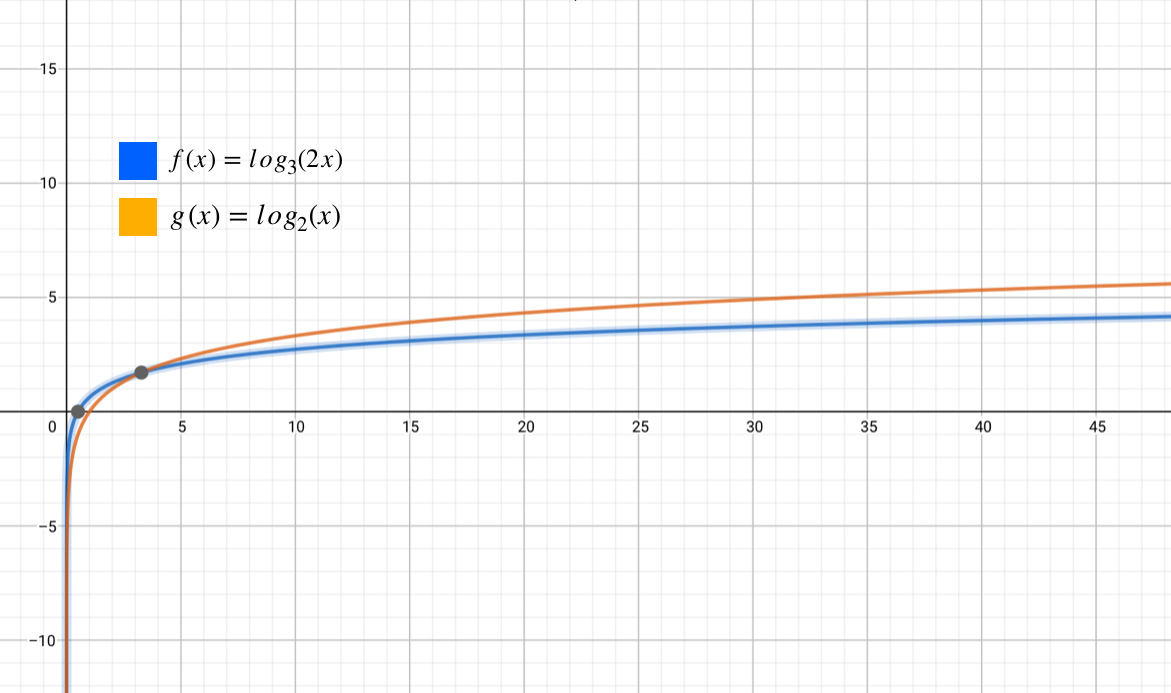
\includegraphics[scale=0.3]{grafica_log.jpg}
        \caption{Gráfica de $log_3(2n)$ vs $log_2(n)$}
    \end{figure}
    

\end{itemize}

\item Aplicación al calculo de la mediana en streaming
\begin{enumerate}
\item Demostrar que el algoritmo propuesto calcula bien el valor mediano.
\item Hacer un análisis de complejidad del algoritmo (puede venir este análisis como comentario en el
código).
\end{enumerate}
\textbf{Respuesta:}
\\
(a) Para la implementación del montículo thmin, como este debe tener en la raíz el elemento mínimo de los datos mayores o iguales a la media, se uso la misma implementación que para un montículo con el máximo en la raíz, con la diferencia que al insertar un nuevo dato se guardo con signo negativo, esto es posible por la propiedad que para un conjunto de números $A$, el $\inf A = -\sup -A$. Para obtener el mínimo de los valores mayores o iguales que la media, se obtuvo el máximo de thmin y se multiplico por -1.

Por construcción de los  montículos, la diferencia en los tamaños es a lo más uno, si ambos montículos tienen tamaño $n$, entonces si se ordenan todos los números, sea $m = getMax(thmax)$, como $m$ es el mayor de los n números en thmax, si los ordenamos, m estaría en la posición n, luego si $M=-getMax(thmin)$, $M$ es el menor de los $n$ números en thmin, y como los elementos de thmin son mayores que los de thmax, si los $2n$ números son ordenados de menor a mayor, $M$ estaría en la posición $n+1$, como en total son $2n$ numeros la mediana es el promedio de los dos del centro que son presisamente $m$ y $M$.

Si un montículo tiene $n$ elementos y el otro tiene $n+1$, supongamos sin pérdida de generalidad que thmax tiene un elemento más, entonces si ordenamos los $2n+1$, $m = getMax(thmax)$ es el mayor de los primeros $n+1$ números, por lo tanto está en la posición del centro, lo que implica que $m$ es la mediana.

(b) Si suponemos que ya se han ingresado $n$ datos y queremos ingresar uno más tendríamos que analizar dos casos, uno donde $n$ es par y otro impar.\\
Si  $n$ es par los montículos max y min tienen la misma cantidad de elementos,tendríamos que hacer las comparaciones del dato a ingresar con la mediana (lo cual tiene un costo constante) y después solo necesitamos mandar llamar la función insert, la cual tiene un costo de $O(log_3 (2n))$, de ahí en fuera todas son constantes que se pueden ignorar. 
\\
Si $n$ es impar tendríamos que verificar en cuál de los montículos tiene mayor longitud, lo cual tiene un costo constante, después realiza las comparaciones del dato a insertar con la mediana, lo cual también tiene un costo constante, en el peor de los casos tendrá que remover la raíz de alguno de los montículos, asignarla a una variable temporal, insertar esta variable temporal en el otro montículo para después insertar el dato en el montículo al que le quitamos la raíz, todo esto tiene un costo de $log_3(2n)+log_3(2n)+log_3(2n)+c=3log_3(2n)+c$ donde $c$ es el número de operaciones constantes, pero por propiedades de “gran O” esto termina siendo de orden $O(log(n))$.
\\ 
Por lo que el método $theap\_median$ tiene una complejidad de $O=(log(n))$

\end{enumerate}

\end{document}  
